%%%%%%%%%%%%%%%%%%%%%%%%%%%%%%%%%%%%%%%%%%%%%%%%%%%%%%%%%%
%   Autoren:
%   Prof. Dr. Bernhard Drabant
%   Prof. Dr. Dennis Pfisterer
%   Prof. Dr. Julian Reichwald
%%%%%%%%%%%%%%%%%%%%%%%%%%%%%%%%%%%%%%%%%%%%%%%%%%%%%%%%%%

%%%%%%%%%%%%%%%%%%%%%%%%%%%%%%%%%%%%%%%%%%%%%%%%%%%%%%%%%%
%	ANLEITUNG: 
%   1. Ersetzen Sie firmenlogo.jpg im Verzeichnis img
%   2. Passen Sie alle Stellen im Dokument an, die mit 
%      @stud 
%      markiert sind
%%%%%%%%%%%%%%%%%%%%%%%%%%%%%%%%%%%%%%%%%%%%%%%%%%%%%%%%%%

%%%%%%%%%%%%%%%%%%%%%%%%%%%%%%%%%%%%%%%%%%%%%%%%%%%%%%%%%%
%	ACHTUNG: 
%   Für das Erstellen des Literaturverzeichnisses wird das 
%   modernere Paket biblatex in Kombination mit biber 
%   verwendet - nicht mehr das ältere Paket BibTex!
%
%   Bitte stellen Sie Ihre TeX-Umgebung entsprechend ein (z.B. TeXStudio): 
%   Einstellungen --> Erzeugen --> Standard Bibliographieprogramm: biber
%%%%%%%%%%%%%%%%%%%%%%%%%%%%%%%%%%%%%%%%%%%%%%%%%%%%%%%%%%

\documentclass[fontsize=12pt,BCOR=5mm,DIV=12,parskip=half,
               listof=entryprefix,paper=a4,toc=bibliography,toc=listof,pointlessnumbers]{scrreprt}
               
\makeindex

%% Elementare Pakete, Konfigurationen und Definitionen werden geladen (gegebenenfalls anpassen)
% !TEX root =  master.tex

%%%%%%%%%%%%%%%%%%%%%%%%%%%%%%%%%%%%%%%%%%%%%%%%%%%%%%%%%%%%%%%%%%
%	ANLEITUNG: 
% Passen Sie gegebenenfalls alle Stellen im Dokument an, die mit 
% @stud 
% markiert sind.
%%%%%%%%%%%%%%%%%%%%%%%%%%%%%%%%%%%%%%%%%%%%%%%%%%%%%%%%%%%%%%%%%%

\usepackage{makeidx}                  % allows index generation
\usepackage{listings}	                %Format Listings properly
\usepackage{lipsum}                   % Blindtext
\usepackage{graphicx}                 % use various graphics formats
\usepackage[german]{varioref}         % nicer references \vref
\usepackage{caption}	                % better Captions
\usepackage{booktabs}                 % nicer Tabs
\usepackage[hidelinks=true]{hyperref} % keine roten Markierungen bei Links
\usepackage{fnpct}                    % Correct superscripts 
\usepackage{calc}                     % Used for extra space below footsepline, in particular
\usepackage{array}
\usepackage{chngcntr}
\usepackage{acronym}
\usepackage{algorithm}
\usepackage{algpseudocode}
\usepackage{setspace}

\usepackage{amsmath}

%% Schriftarten- und Zeichenpakete
\usepackage[T1]{fontenc}
\usepackage[utf8]{inputenc}
\usepackage{minted}
\usepackage[usenames,dvipsnames]{xcolor}


%%
%% @stud
%%
%%	FONT SELECTION: Schriftarten und Schriftfamilie
%%%%%%%%%%%%%
%% SCHRIFTART
%%%%%%%%%%%%%
% 0) without decomment: normal font families 
% ...
% 1) Latin Modern 
%\usepackage{lmodern}        
% 2) Times 
%\usepackage{mathptmx}         
% 3) Helvetica
%\usepackage[scaled=.92]{helvet} 
%%%%%%%%%%%%%%%%%%
%%	SCHRIFTFAMILIE
%%%%%%%%%%%%%%%%%%
% ohne Serifen
\renewcommand*{\familydefault}{\sfdefault}
\addtokomafont{disposition}{\sffamily}
%
% mit Serifen
%\renewcommand*{\familydefault}{\rmdefault}
%\addtokomafont{disposition}{\rmfamily}
%
% Typewriter
%\renewcommand*{\familydefault}{\ttdefault}
%\addtokomafont{disposition}{\ttfamily}

%%
%% @stud
%%
%% LANGUAGE SETTINGS
\usepackage[ngerman]{babel} 	        % german language
\usepackage[german=quotes]{csquotes} 	% correct quoting using \enquote{}
%\usepackage[english]{babel}          % english language
%\usepackage{csquotes} 	              % correct quoting using \enquote{}

%%
%% @stud
%%
%% Uncomment the following lines to support hard URL breaks in bibliography 
%\apptocmd{\UrlBreaks}{\do\f\do\m}{}{}
%\setcounter{biburllcpenalty}{9000}% Kleinbuchstaben
%\setcounter{biburlucpenalty}{9000}% Großbuchstaben

%%
%% @stud
%%
%% FOOTNOTES: Count footnotes over chapters
%\counterwithout{footnote}{chapter}

%	ACRONYMS
\makeatletter
\@ifpackagelater{acronym}{2015/03/20}
{\renewcommand*{\aclabelfont}[1]{\textbf{{\acsfont{#1}}}}}{}
\makeatother

%	LISTINGS
\renewcommand{\lstlistingname}{Quelltext}
\renewcommand{\lstlistlistingname}{Quelltextverzeichnis}
\lstset{numbers=left,
	numberstyle=\tiny,
	captionpos=b,
	basicstyle=\ttfamily\small}

%	ALGORITHMS
\renewcommand{\listalgorithmname}{Algorithmenverzeichnis }
\floatname{algorithm}{Algorithmus}

%	PAGE HEADER / FOOTER
%	Warning: There are some redefinitions throughout the master.tex-file!  DON'T CHANGE THESE REDEFINITIONS!
\RequirePackage[automark]{scrlayer-scrpage}
%alternatively with separation lines: \RequirePackage[automark,headsepline,footsepline]{scrlayer-scrpage}

\renewcommand{\chaptermarkformat}{}
\RedeclareSectionCommand[beforeskip=0pt]{chapter}
\clearscrheadfoot

%\ifoot[\rule{0pt}{\ht\strutbox+\dp\strutbox}DHBW Mannheim]{\rule{0pt}{\ht\strutbox+\dp\strutbox}DHBW Mannheim}
\ofoot[\rule{0pt}{\ht\strutbox+\dp\strutbox}\pagemark]{\rule{0pt}{\ht\strutbox+\dp\strutbox}\pagemark}
\ohead{\headmark}

\newcommand{\TitelDerArbeit}[1]{\def\DerTitelDerArbeit{#1}\hypersetup{pdftitle={#1}}}
\newcommand{\AutorDerArbeit}[1]{\def\DerAutorDerArbeit{#1}\hypersetup{pdfauthor={#1}}}
\newcommand{\Kurs}[1]{\def\DieKursbezeichnung{#1}}
\newcommand{\Studiengangsleiter}[1]{\def\DerStudiengangsleiter{#1}}
\newcommand{\WissBetreuer}[1]{\def\DerWissBetreuer{#1}}
\newcommand{\Bearbeitungszeitraum}[1]{\def\DerBearbeitungszeitraum{#1}}
\newcommand{\Abgabedatum}[1]{\def\DasAbgabedatum{#1}}
\newcommand{\Matrikelnummer}[1]{\def\DieMatrikelnummer{#1}}
\newcommand{\Studienrichtung}[1]{\def\DieStudienrichtung{#1}}
\newcommand{\ArtDerArbeit}[1]{\def\DieArtDerArbeit{#1}}
\newcommand{\Literaturverzeichnis}{Literaturverzeichnis}

\newcommand{\settingBibFootnoteCite}{
	\setlength{\bibparsep}{\parskip}		  % Add some space between biblatex entries in the bibliography
	\addbibresource{bibliography/bibliography.bib}	    % Add file bibliography.bib as biblatex resource
	\DefineBibliographyStrings{ngerman}{andothers = {{et\,al\adddot}},}
}

\newcommand{\setTitlepage}{
	% !TEX root =  master.tex
\begin{titlepage}
\begin{minipage}{\textwidth}
		\vspace{-2cm}
		
\includegraphics{\imagedir/logo.jpg}
\end{minipage}
\vspace{1em}
%\sffamily
\begin{center}
	{\textsf{\large Duale Hochschule Baden-W\"urttemberg Mannheim}}\\[4em]
	{\textsf{\textbf{\large{\DieArtDerArbeit}arbeit}}}\\[6mm]
	{\textsf{\textbf{\Large{}\DerTitelDerArbeit}}} \\[1.5cm]
	{\textsf{\textbf{\large{}Studiengang Informatik}}\\[6mm]
	\textsf{\textbf{Studienrichtung \DieStudienrichtung}}}\vspace{10em}
	
	\begin{minipage}{\textwidth}
		\begin{tabbing}
		Wissenschaftliche(r) Betreuer(in): \hspace{0.85cm}\=\kill
		Verfasser(in): \> \DerAutorDerArbeit \\[1.5mm]
		Matrikelnummer: \> \DieMatrikelnummer \\[1.5mm]
		Kurs: \> \DieKursbezeichnung \\[1.5mm]
		Studiengangsleiter: \> \DerStudiengangsleiter \\[1.5mm]
		Wissenschaftliche(r) Betreuer(in): \> \DerWissBetreuer \\[1.5mm]
		Bearbeitungszeitraum: \> \DerBearbeitungszeitraum\\[1.5mm]
%		alternativ:\\[1.5mm]
%		Eingereicht: \> \DasAbgabedatum	
		\end{tabbing}
	\end{minipage}
\end{center}
\end{titlepage}
	\pagenumbering{roman} % Römische Seitennummerierung
	\normalfont
}

%%
%% @stud
%%
\newcommand{\settingLists}{
	%	Inhaltsverzeichnis
	\tableofcontents
	%	Abbildungsverzeichnis
	\listoffigures
	%	Tabellenverzeichnis
	% \listoftables
	%	Listingsverzeichnis / Quelltextverzeichnis
	% \lstlistoflistings
	% Algorithmenverzeichnis
	% \listofalgorithms
}

\newcommand{\initializeText}{
	\clearpage
	\ihead{\chaptername~\thechapter} % Neue Header-Definition
	\pagenumbering{arabic}           % Arabische Seitenzahlen
}

\newcommand{\initializeBibliography}{
	\ihead{}
	\printbibliography[title=\Literaturverzeichnis]
	\cleardoublepage
}

\newcommand{\initializeAppendix}{
	\appendix
	\ihead{\appendixname~\thechapter}
}



%%
%% @stud
%%
%% PERSÖNLICHE ANGABEN (BITTE VOLLSTÄNDIG EINGEBEN zwischen den Klammern: {...})
%%
\ArtDerArbeit{Seminar} % "Bachelor" oder "Projekt" wählen
\TitelDerArbeit{Analyse der Lösbarkeit von Instanzen des 15-Puzzzles mit Implementierung}
\AutorDerArbeit{Kai Fischer, Max Stubenbord}
\Kurs{TINF18AI1}
\Studienrichtung{angewandte Informatik}
\Matrikelnummer{3683691, 5379506}
\Studiengangsleiter{Prof. Dr. Holger Hofmann}
\WissBetreuer{Prof. Dr. Karl Stroetmann}
\Bearbeitungszeitraum{24.03.2021 -- 11.06.2021}
\Abgabedatum{11.06.2021}

%%
%% @stud
%%
%% BIBLIOGRAPHY (@stud: Bibliographie-Stil wählen - Position und Indizierung)
%%  Auswahl zwischen: 
%%   NUMERIC Style
%%   IEEE Style
%%   ALPHABETIC Style
%%   HARVARD Style
%%   CHICAGO Style 
%%   (oder eigenen zulässigen Stil wählen) 
%%
%%%%%%%%%%%%%
%% Zitierstil
%%%%%%%%%%%%%
% NUMERIC Style - e. g. [12]
\newcommand{\indextype}{numeric} 
%
% IEEE Style - numeric kind of style 
%\newcommand{\indextype}{ieee} 
%
% ALPHABETIC Style - e. g. [AB12]
%\newcommand{\indextype}{alphabetic} 
%
% HARVARD Style 
%\newcommand{\indextype}{apa} 
%
% CHICAGO Style 
%\newcommand{\indextype}{authoryear}
%
%%%%%%%%%%%%%%%%%%%%%%
%% Position des Zitats
%%%%%%%%%%%%%%%%%%%%%%
\newcommand{\position}{inline} 
%
% (!!) FOOTNOTE POSITION NOT RECOMMENDED IN MINT DOMAIN:
%\newcommand{\position}{footnote}

%% Final: Setzen des Zitierstils und der Zitatposition
\usepackage[backend=biber, autocite=\position, style=\indextype]{biblatex} 	
\settingBibFootnoteCite

%%
%% Definitionen und Commands
%%
\newcommand{\abs}{\par\vskip 0.2cm\goodbreak\noindent}
\newcommand{\nl}{\par\noindent}
\newcommand{\mcl}[1]{\mathcal{#1}}
\newcommand{\nowrite}[1]{}
\newcommand{\NN}{{\mathbb N}}
\newcommand{\imagedir}{img}

\makeindex

\begin{document}

\setTitlepage

%%%%%%%%%%%%%%%%%%%%%%%%%%%%%%%%%%%%%%%%%%%%%%%%%%%%%%%%%%%%%%%%%%%%%%%%%%%%%%%%%%%%%%%%%%
% KAPITEL UND ANHÄNGE
%
% @stud:
%   - nicht benötigte: auskommentieren/löschen
%   - neue: bei Bedarf hinzufügen mittels input-Kommando an entsprechender Stelle einfügen
%%%%%%%%%%%%%%%%%%%%%%%%%%%%%%%%%%%%%%%%%%%%%%%%%%%%%%%%%%%%%%%%%%%%%%%%%%%%%%%%%%%%%%%%%%

%%%%%%%%%%%%%%%%%%%%%%%%%%%%%%%%%%%
% EHRENWÖRTLICHE ERKLÄRUNG
%
% @stud: ewerkl.tex bearbeiten
%
% !TEX root =  master.tex
\clearpage
\chapter*{Ehrenwörtliche Erklärung}

% Wird die folgende Zeile auskommentiert, erscheint die ehrenwörtliche
% Erklärung im Inhaltsverzeichnis.

% \addcontentsline{toc}{chapter}{Ehrenwörtliche Erklärung}
Ich versichere hiermit, dass ich die vorliegende Arbeit mit dem Titel ``\textit{\DerTitelDerArbeit}'' selbstständig verfasst und 
keine anderen als die angegebenen Quellen und Hilfsmittel benutzt habe. Ich versichere zudem, dass die eingereichte elektronische 
Fassung mit der gedruckten Fassung übereinstimmt.

\vspace{3cm}
Ort, Datum \hfill \DerAutorDerArbeit

%%%%%%%%%%%%%%%%%%%%%%%%%%%%%%%%%%%

%%%%%%%%%%%%%%%%%%%%%%%%%%%%%%%%%%%
% SPERRVERMERK
%
% @stud: nondisclosurenotice.tex bearbeiten
%
%% !TEX root =  master.tex
\chapter*{Sperrvermerk}

\begin{center}
\fbox{
		\begin{minipage}{33em}
			\textbf{Ein Sperrvermerk sollte nur bei berechtigtem Bedarf gesetzt werden!\\[10pt] 
				Beachten Sie, dass mit Sperrvermerk	versehene Arbeiten nicht für weitere wissenschaftliche Zwecke 
				außerhalb des Firmenkontextes oder zur Publikation verwendet werden dürfen.\\[10pt]
				Wir empfehlen, wenn m\"oglich, auf den Sperrvermerk zu verzichten.\\[10pt]
				Besprechen Sie diese Problematik mit Ihrer Firma!}
		\end{minipage}
}
\end{center}

(Mustertext) Der Inhalt dieser Arbeit darf weder als Ganzes noch in Auszügen Personen außerhalb des Prüfungsprozesses 
und des Evaluationsverfahrens zugänglich gemacht werden, sofern keine anders lautende Genehmigung der Ausbildungsstätte vorliegt. 

\cleardoublepage

%%%%%%%%%%%%%%%%%%%%%%%%%%%%%%%%%%%

%%%%%%%%%%%%%%%%%%%%%%%%%%%%%%%%%%%
%	KURZFASSUNG
%
% @stud: acknowledge.tex bearbeiten
%
% !TEX root =  master.tex
\chapter*{Danksagung}

Ein besonderer Dank geht an Prof. Dr. Stroetmann f"ur die Erm"oglichung einer alternativen Pr"ufungsleistung. Wie wir w"ahrend der Corona-Zeit festgestellt haben, ist ein solches Engagement nicht selbstverst"andlich.\\
Abschlie"send wollen wir uns auch bei dem Kurs TINF18AI1 bedanken f"ur die faire und strukturierte Verteilung der Themen.



%%%%%%%%%%%%%%%%%%%%%%%%%%%%%%%%%%%

%%%%%%%%%%%%%%%%%%%%%%%%%%%%%%%%%%%
%	KURZFASSUNG
%
% @stud: abstract.tex bearbeiten
%
% !TEX root =  master.tex
\chapter*{Abstract}

The 15-puzzle first gained public attention in the 1870s when Sam Loyd promised $\$1000$ in prize money to anyone who could solve his puzzle, which became known as the 14-15 puzzle.\\
It was not until nearly a decade later that authors of the American Journal of Mathematics published a proof that the puzzle is unsolvable.
Today, the 15-puzzle is a classic use case when it comes to modelling algorithms with heuristics, such as \textit{A*} or \textit{IDA*}.\\
The main purpose of this work is to outline and implement the algorithm for checking the solvability of an instance of the 15-puzzle.
This algorithm is based on Bradlow's approach where a puzzle is considered solvable, if the parity of the transposition count and the manhattan distance of the blank field match.\\The In the process written source-code can be found within the appendix. To test this implementation, an evaluation of specific test-cases is conducted.\\
Altough the algorithm specifies the solvability for a given puzzle instance, it remains uncertain how many steps are required to obtain this solution. Hence the algorithm provides no indicator for computing time.

%%%%%%%%%%%%%%%%%%%%%%%%%%%%%%%%%%%

%%%%%%%%%%%%%%%%%%%%%%%%%%%%%%%%%%%
% VERZEICHNISSE
%
% @stud: ggf. nicht benötigte Verzeichnisse auskommentieren/löschen in Def. von \settingLists in config.tex
%
\settingLists
%%%%%%%%%%%%%%%%%%%%%%%%%%%%%%%%%%%

%%%%%%%%%%%%%%%%%%%%%%%%%%%%%%%%%%%
% ABKÜRZUNGSVERZEICHNIS
%
% @stud: acronyms.tex bearbeiten
%
% !TEX root =  master.tex
\clearpage
\chapter*{Abkürzungsverzeichnis}	
\addcontentsline{toc}{chapter}{Abkürzungsverzeichnis}

\begin{acronym}[XXXXXXX]
	\acro{ad}[AD]{Archiv für Diplomatik, Schriftgeschichte, Siegel- und Wappenkunde}
	\acro{BMBF}{Bundesministerium für Bildung und Forschung}	
	\acro{DHBW}{Duale Hochschule Baden-Württemberg}
	\acro{ecu}[ECU]{European Currency Unit}
	\acro{eu}[EU]{Europäische Union}
	\acro{RDBMS}[RDBMS]{Relational Database Management System}
\end{acronym}
%%%%%%%%%%%%%%%%%%%%%%%%%%%%%%%%%%%

\initializeText
\onehalfspacing

%%%%%%%%%%%%%%%%%%%%%%%%%%%%%%%%%%%
% KAPITEL
%
% @stud: einzelne Kapitel bearbeiten und eigene Kapitel hier einfügen
%
% Einleitung
% !TEX root =  master.tex
\chapter{Einleitung}

\nocite{*}

Dieses Kapitel enthält die Einleitung mit ihren verschiedenen Abschnitten/Sections und Unterabschnitten.

\section{Beispiel Abschnitt: \LaTeX-Installation}

Zur Verwendung von \LaTeX-Installation einer Distribution z.~B.~TeXLive, MikTex etc.~sowie eines Editors z.~B.~TeXStudio, TeXnicCenter etc.~notwendig.

Installieren Sie zun\"achst die Distribution und anschließend den Editor. Beim ersten Start des Editors \"offnet sich ein 
Konfigurationsassistent, der zun\"achst nach dem Pfad der installierten Distribution fragt. 

Nach der Installation können k\"onnen Einstellungen z.~B.~f\"ur einen PostScript-Viewer gemacht werden. 
Dieser Schritt kann ohne Weiteres \"ubersprungen werden. Entscheidend sind die Einstellungen f\"ur den pdf-Viewer. 

Jetzt kann \LaTeX~verwendet werden. Um die Ausgabe eines Dokumentes zu erzeugen, muss das Dokument kompiliert werden (Ausgabe >
Aktives Dokument > Erstellen und betrachten).

\subsection{Beispiel Unterabschnitt: Aufbau eines \LaTeX-Dokuments}

Ein \LaTeX-Dokument besteht in der Regel aus folgenden Komponenten:
\begin{itemize}
	\item Pr\"aambel
	\item Titelseite
	\item Textteil
\end{itemize}

\subsubsection{Beispiel Unterabschnitt auf zweiter Ebene: Pr\"aambel}
In der Pr\"aambel werden global die Einstellungen f\"ur das gesamte Dokument definiert. Hierbei k\"onnen z.~B.~die Seitenr\"ander, 
der Zeilenabstand oder auch die Sprache f\"ur die Silbentrennung festgelegt werden. In der ersten Zeile eines jeden Dokumentes wird dabei
immer die zu verwendende Klasse festgelegt. Standardm\"aßig kann hier die Artikel-Klasse gew\"ahlt werden:

\texttt{\textbackslash documentclass[12pt,titlepage]\{article\}}

In den eckigen Klammern wird dabei u.a. die Standardschriftgr\"o\ss e f\"ur das gesamte Dokument festgelegt. 

Au\ss erdem werden in der Pr\"aambel die f\"ur das Dokument ben\"otigten Pakete festgelegt. Gebr\"auchlich sind vor allem folgende Pakete:
{\texttt{
\begin{itemize}
	\item \textbackslash usepackage[ngerman]\{babel\}
	\item \textbackslash usepackage[latin1]\{inputenc\}
	\item \textbackslash usepackage\{color\}
	\item \textbackslash usepackage[a4paper]\{geometry\}
	\item \textbackslash usepackage\{amssymb\}
	\item \textbackslash usepackage\{amsthm\}
	\item \textbackslash usepackage\{graphicx\}
\end{itemize}
}

Im vorliegenden Fall werden die Pakete in der Konfigurationsdatei \texttt{config.tex} festgelegt, deren Inhalt durch 
\texttt{\textbackslash input\{config\}} in das Hauptdokument \texttt{master.tex} inkludiert wird.

\subsubsection{Beispiel Unterabschnitt auf zweiter Ebene: Titelseite}

Nachdem die Dokumenten-Klasse und die zu verwendenden Pakete festgelegt worden sind,
folgt die Titelseite. Da die Titelseite bereits Teil des eigentlichen Dokuments ist, muss ihr
unbedingt der Befehl \texttt{\textbackslash begin\{document\}} vorausgehen. Am Ende des Dokuments sollte der Befehl
\texttt{\textbackslash end\{document\}} gesetzt werden. Alles was nach diesem Befehl steht, wird vom Compiler nicht mehr beachtet.

\subsubsection{Beispiel Unterabschnitt auf zweiter Ebene: Textteil}

Der Textteil beinhaltet nun den eigentlichen Text des Dokuments.


% mehrere Grundlagen- und Forschungs-Kapitel
% !TEX root =  master.tex
\chapter{Grundlagen}
In diesem Kapitel werden die theoretischen Grundlagen und Gedanken für die Umsetzung im nächsten Kapitel \ref{chap:Implementation} vorgestellt. Die Lösung und das Vorgehen basieren maßgeblich auf dem Beitrag \afz{\MaxLink{https://www.youtube.com/watch?v=YI1WqYKHi78}{Why is this Puzzle Impossible? - Numberphile}} von Herrn Steven Bradlow zur Lösbarkeit des \afz{14-15 puzzles} aus der Einleitung auf dem Youtube Kanal \afz{Numberphile} \autocite{Unsolvable-14-15-Numberphile-YT:online}.%
%
\section{Puzzle zu Listen wandeln} % (fold)
\label{sec:PuzzleToList}
Der Lösungsansatz aus \autocite{Unsolvable-14-15-Numberphile-YT:online} basiert auf Permutationen. Um 4x4 Puzzle besser auf Permutationen untersuchen zu können, werden die Puzzle als Listen von Zahlen dargestellt. Dazu werden die Inhalte der Zellen des Puzzle zeilenweise hintereinander in eine Liste geschrieben. Die Leerstelle, auch als \afz{blank} beschrieben, wird dabei als Zahl \afz{0} interpretiert.
Der Zustand des Puzzle aus Abb.\ref{fig:Perm_puzzle_start_Pic}
\begin{figure}[H]
	\centering
	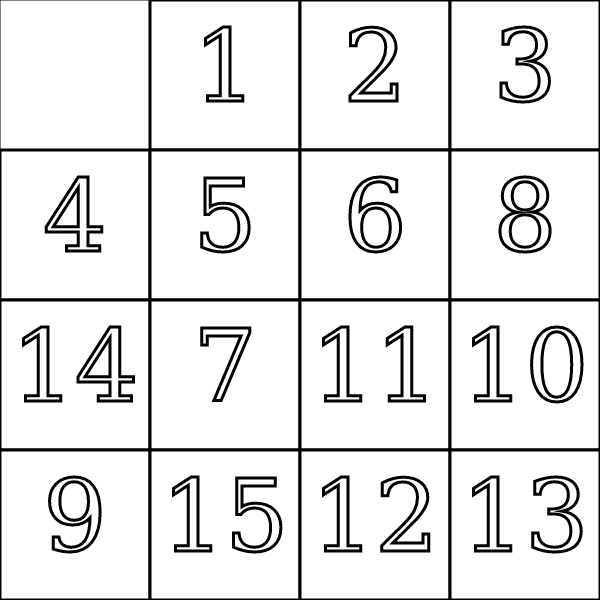
\includegraphics[width=.5\textwidth,keepaspectratio]{img/Start_Puzzle2.png}
	\captionsetup{format=hang}
	\caption{Beispiel Zustand eines 4x4-Puzzle \label{fig:Perm_puzzle_start_Pic}}
\end{figure}
\begin{minipage}{\linewidth}
	wird als Liste aus Zahlen wie folgt dargestellt:
	\begin{center}
		$State = \{0,1,2,3,4,5,6,8,14,7,11,10,9,15,12,13\}$
	\end{center}
\end{minipage}\WNL%
Wichtig ist bei der Betrachtung der lösbaren Puzzle und des Vorgehens der Lösung aus \autocite{Unsolvable-14-15-Numberphile-YT:online} aber auch anderer verfügbarer Quellen \autocite{solving-15-puzzle-lvi:article,geeksforgeeks:online,archer-15-puzzle:article}, dass die Bezeichnung der Leerstelle oder die Art der Konvertierung eines Puzzle zu einer Liste variiert. Die meisten Lösungen sehen den Zielzustand aus Abb.\ref{fig:Perm_puzzle_end_allOther} vor, wobei die Leerstelle dann die Nummer \afz{16} trägt. Um mit den Darstellungen von Herrn Stroetmann aus dem Vorlesungsskript \autocite{github-stroetmann:online} übereinzustimmen, wird der Zielzustand aus Abb.\ref{fig:Perm_puzzle_end_stroet} angestrebt, bei dem die Leerstelle die Nummer \afz{0} trägt.\\
%
\begin{minipage}{\linewidth}
	\begin{minipage}[t]{0.45\linewidth}
		\begin{figure}[H]
			\centering
			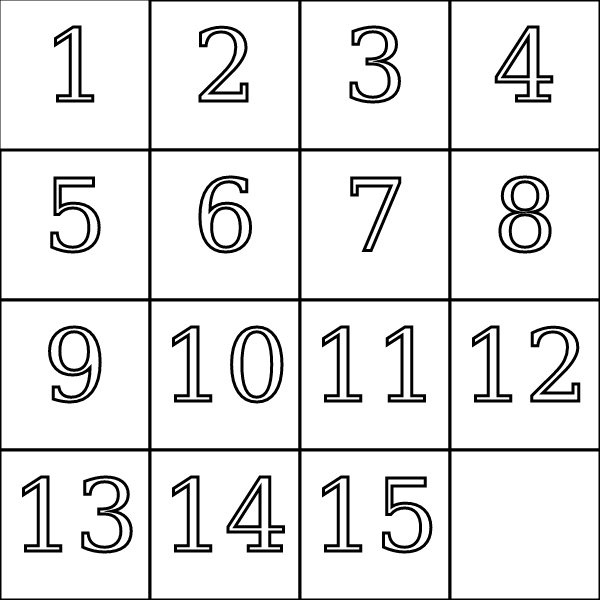
\includegraphics[width=\linewidth,keepaspectratio]{img/End_Puzzle_AO.png}
			\captionsetup{format=plain, indention=0pt}
			\caption{Häufig verwendeter Zielzustand eines 4x4-Puzzle \label{fig:Perm_puzzle_end_allOther}}
		\end{figure}
	\end{minipage}
	\hfill
	\begin{minipage}[t]{0.45\linewidth}
		\begin{figure}[H]
			\centering
			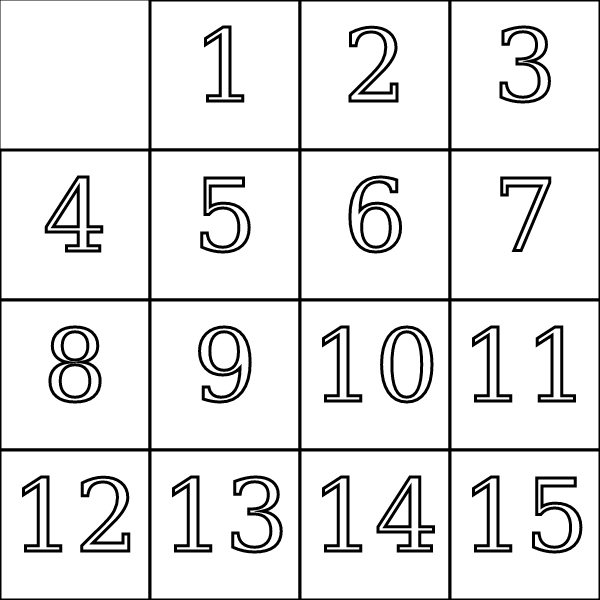
\includegraphics[width=\linewidth,keepaspectratio]{img/End_Puzzle_Stroetmann.png}
			\captionsetup{format=plain, indention=0pt}
			\caption{\label{fig:Perm_puzzle_end_stroet}Verwendeter Zielzustand eines 4x4-Puzzles aus dem Skript von Herrn Stroetmann \autocite{github-stroetmann:online}}
		\end{figure}
	\end{minipage}
\end{minipage}\WNL%

\section{Zustände als Permutationen} % (fold)
\label{sec:Permutation}
Die Grund-Idee der Lösbarkeitsüberprüfung von Bradlow basiert auf dem Vergleichen der Paritäten zwischen benötigten Transpositionen und benötigter Züge zum Verrücken der Leerstelle. Im Folgenden wird die Idee aus seinem Beitrag \autocite{Unsolvable-14-15-Numberphile-YT:online} zusammengefasst vorgestellt.\WNL

Die Vorstellung des Verfahrens beginnt Bradlow damit die Puzzle wie in der vorherigen Sektion in Zahlen Reihen zu wandeln. Durch das Vertauschen von 2 beliebigen Zahlen aus dieser Zahlenreihe entsteht eine Permutation der vorherigen Reihe. Auf diese Weise sei jeder möglicher Zustand in dem sich das Puzzle befinden kann als eine Permutation einer zugrundeliegenden aufsteigend sortieren Zahlenreihe zu sehen. Für diese Permutationen beschreit er die folgenden zwei Eigenschaften:
\begin{enumerate}
	\item[\textbf{E1}] Jede dieser Permutationen lässt sich nur durch das Nutzen von Transpositionen, also dem Vertauschen von Zwei Elementen aus der Liste, während die restlichen gleich bleiben, in eine andere Permutation überführen \cite[Vgl.][7min,07sec]{Unsolvable-14-15-Numberphile-YT:online}.
	\item[\textbf{E2}] Die Anzahl der Schritte, die für das Überführen einer Permutation in eine andere Permutation mithilfe von Transpositionen benötigt wird, ist nicht Festgelegt, aber die Parität dieser Zahl ist fest \cite[Vgl.][10min,13sec]{Unsolvable-14-15-Numberphile-YT:online}.
\end{enumerate}
Basierend auf diesen Eigenschaften fährt er fort, dass die Parität der Anzahl notwendiger Transpositionen durch das zielgerichtete Tauschen der Zahlen, mit dem ziel einer aufsteigen sortieren Zahlenreihe, ermittelt werden kann. Wie in der vorherigen Sektion beschrieben, sieht auch Bradlow die sortierte Zahlenreihe
\begin{center}
	$Goal_{Bradlow} = {1,2,3,4,5,6,7,8,9,10,11,12,13,14,15,16}$
\end{center}
als Abbild des Zielzustandes vor. Daher ist in seinem Vortrag das Ziel der Transpositionen die aufsteigend sortierte Liste. Durch E1 ist sicher gestellt, dass die sortiere Liste erreicht werden kann. E2 begründet, dass die Parität der für die Sortierung notwendigen Transpositionen mit der Parität der notwendigen Züge, wenn das Puzzle lösbar ist, übereinstimmt, obwohl die Regeln des Puzzles nicht betrachtet und somit möglicherweise nicht eingehalten werden.\WNL
Im zweiten Schritt der Lösbarkeitsüberprüfung ermittelt Bradlow die Parität der notwendigen legalen Züge zum Überführen der Leerstelle aus dem Startzustand zum Zielzustand. Dabei ist ebenfalls jeder einzelne Zug als eine Transposition zu sehen.\WNL%
Lösbar ist ein Puzzle nach Bradlow dann, wenn die ermittelten Paritäten übereinstimmen. Denn nach E2 sind die Paritäten festgelegt und können nicht verändert werden. Die Parität der Leerstellen Bewegung ist Legal, während Parität der notwendigen zur Sortierung notwendigen Züge nur hypothetisch sind. stimmen die Paritäten nicht über ein existiert nach E2 keine Möglichkeit beide Ziele, also die Sortierung ebenso wie das einhalten Zugregeln einzuhalten. 
\WNL
In der nächsten Sektion wird dieses Verfahren an einem Beispiel schrittweise durchgegangen.
\WNL
Für die Sektion \ref*{cha:Umsetzung}, soll noch erwähnt werden, dass sich die Leerstelle nur horizontal und vertikal \afz{bewegen} darf und sich die Anzahl der Züge so mithilfe der Manhattan-Distanz ermitteln lässt.


\section{Kontext Vorlesung + Abgrenzung} % (fold)
\label{cha:Kontext Vorlesung}

% chapter Kontext Vorlesung (end)
\section{Sortieralgorithmen} % (fold)
\label{cha:Sortieralgorithmen}
Mit Ordnung?!
% chapter Sortieralgorithmen (end)
% Endzustände sind nicht ineinander überführbar
% Betrachtung von 2x2 Puzzle um zu zeigen dass es immer 2pfade gibt
% Betrachtung des Loyd Puzzles
% Betrachtung der einen Vorgegebenen Lösung von Herrn Stroetmann 




% !TEX root =  master.tex
\chapter{Implementation}
\label{chap:Implementation}
\section{Umsetzung} % (fold)
\label{cha:Umsetzung}
\texttt{Der vollst"andige Quellcode ist im Anhang unter \ref{code:validate-15-puzzle:py} zu finden.}\\\\
Zur Umsetzung wird zu erst eine Datenstruktur definiert, in welcher die Instanzen des 15-Puzzles ausgewertet werden. Hierf"ur werden Tupel von Tupeln verwendet.
Anschlie"send ist die gernerelle Idee, wie auch schon in \texttt{kais abschnitt?} vorgestellt zu schauen, ob die Anzahl der Permutationen bei der Datenstruktur als $1$-Dimensionale Liste und der Abstand des Blank-Feldes vom Start- zum Zielzustand die gleiche Parit"at besitzen.
Ist diese gleich, so ist das Puzzle l"osbar, vice versa unl"osbar.\\
Spannend ist hier allerdings, dass dies kein Indikator f"ur die Komplexit"at der L"osbarkeit ist. So kann ein l"osbares Puzzle mit den zur Verf"ugung stehenden Algorithmen wie \textit{A*} oder \textit{IDA*} nicht in angemessener Zeit gel"ost werden.\\
Das weitere Vorgehen der Implementierung ist weitesgehend die Bearbeitung von kleinen Teilproblemen, welche sich aus dem eben genannten Vorgehen ergeben.\\
So betrachten wir zun"achst die Anzahl der Permutationen, welche sich in einer Puzzleinstanz befinden. Um diese zu berechnen wird als Datenstruktur eine Liste mit der Dimension 1 ben"otigt.
Anschlie"send muss die Liste durch tauschen der Elemente sortiert werden.
\texttt{n"achsten Satz "uberarbeiten!}\\
Vereinfacht wird dieser Schritt dadurch, dass der L"osungszustand des Puzzles so definiert ist, dass der Index innerhalb der Liste und der Wert des zugeh"origen Elementes identisch sind. Somit kann f"ur jeden Index der entsprechende Wert innerhalb der Liste gesucht werden, sodass eine minimale Anzahl von \textit{swaps} durchgef"uhrt werden. \\Die Anzahl der get"atigten \textit{swaps} liefert uns dann die Anzahl der mindestens durchzuf"uhrenden Permutationen innerhalb der Puzzleinstanz.\\
Die Implementierung ist dabei wie folgt:
\begin{minted}[linenos,breaklines,breakanywhere]{python}
def get_inversion_count(Puzzle: tuple) -> int:
    working_1d_puzzle = to_1d(Puzzle)
    count = 0
    for i in range(len(working_1d_puzzle)):
        if working_1d_puzzle[i] != i:
            count += 1
            swap(i, find_tile_1d(i, working_1d_puzzle), working_1d_puzzle)
    return count
\end{minted}
wobei die Funktion \textbf{to\_1d} definiert ist durch
\vspace{.25cm}
\begin{minted}[breaklines,breakanywhere]{python}
to_1d = lambda Puzzle: [elem for tupl in Puzzle for elem in tupl]
\end{minted}
\vspace{.25cm}
und die Funktion \textbf{swap} durch
\vspace{.25cm}
\begin{minted}[breaklines,breakanywhere]{python}
def swap(idxA, idxB, Puzzle_1d):
    Puzzle_1d[idxA], Puzzle_1d[idxB] = Puzzle_1d[idxB], Puzzle_1d[idxA]
\end{minted}
\vspace{.25cm}
definiert ist.\\
Die Funktion \textbf{find\_tile\_1d} gibt den Index einer 1-Dimensionalen Liste zur"uck, an der das entsprechende Element zu finden ist. Diese ist auch im Anhanhg unter \ref{code:validate-15-puzzle:py} zu finden.\\
Nun muss als n"achstes die Distanz des Blank-Feldes vom Startzustand zum Zielszustand berechnet werden. Wie schon in Abschnitt \ref{sec:Permutation} angesprochen kann die Anzahl der notwendigen Z"uge um das Blank-Feld von der Position im Startzustand zu der Position im Zielzustand zu bewegen durch die Manhattan-Distanz ermittelt werden..\\ Da die $x,y$ Position des Blank-Feldes im Endzustand immer $0,0$ ist, muss diese nicht berechnet werden, wird in der Funktion allerdings auch gesucht, sodass bei einer Erweiterung noch der Endzustand variieren kann.
Sei $x_1,y_2$ nun die Position des Blank-Feldes im Startzustand und $x_2,y_2$ die Position des Blank-Feldes im Endzustand, so ist der Abstand beider Blank-Felder durch \\
\begin{center}
    $\left | x_1 - x_2 \right | + \left | y_1 - y_2 \right |$
\end{center}
definiert.\\
Die dazugeh"orige Funktion \textbf{manhattan} ist auch im Anhang unter \ref{code:validate-15-puzzle:py} zu finden.\\
Abschlie"send wird verglichen, ob die Summe der Distanz und die Anzahl der Permutationen im Startzustand die gleiche Parit"at besitzen. Stimmen die Parit"aten "uberein, so ist die Instanz l"osbar, sind diese unterschiedlich, so ist diese unl"osbar.

% \inputminted[linenos,breaklines,breakanywhere]{python}{../code/15-solvable-v1.py}
% chapter Umsetzung (end)
\section{Testing} % (fold)
\label{cha:Testing}
Um nun verschiedene Puzzleinstanzen und deren L"osbarkeit anhand des Codes zu testen, werden verschiedene Startzust"ande und zu Testzwecken verschiedene Endzust"ande definiert. Anschlie"send werden alle Startzust"ande auf L"osbarkeit des \enquote{normalen} Endzustandes getestet.\\
Um eine verbose Ausgabe zu erm"oglichen, bei der noch die verschiedenen zuvor berechneten Werte ausgegeben werden k"onnen, kann der Funktion, welche die Puzzleinstanzen auf ihre L"osbarkeit pr"uft, noch eine entsprechende verbose Flag mitgegeben werden. Somit kann anhand von bekannten l"osbaren Instanzen "uberpr"uft werden, ob die Implementierung vollst"andig ist.\\
Der Output dieses Testes befindet sich im dazugeh"origen \textcolor{violet}{\href{https://github.com/stubifox/ai-termpaper/blob/main/code/15-solvable-v1.ipynb}{Jupyter-Notebook}}.\\
Diese Puzzle werden dann bspw. in das schon aus der Vorlesung bekannte \textcolor{violet}{\href{https://github.com/karlstroetmann/Artificial-Intelligence/blob/master/Python/1\%20Search/Iterative-Deepening-A-Star-Search.ipynb}{Jupyter-Notebook}} zum L"osen der Instanzen gegeben, so dass geschaut werden kann, ob diese in angemessener Zeit l"osbar sind, und wieviele Z"uge f"ur die jeweilige L"osung gebraucht werden. \\
Ein Screenshot des Outputs findet sich im Anhang unter \ref{app:fig:testing-output}.
Problem hierbei ist, dass nicht jedes als l"osbar einkategorisierte Puzzle auch in angemessener Zeit mit Hilfe des \textit{IDA*} oder \textit{A*} Algorithmus gel"ost werden kann. So ist es durchaus vorgekommen, dass die Schritte zur L"osbarkeit eines Puzzles mehrere Stunden dauern (vgl. \ref{app:fig:1h}), da vorher nicht bekannt ist, wieviele Schritte zur L"osung f"uhren.\\
Somit wei"s man initial nicht, ob das Puzzle richtig einklassifiziert wurde.
% chapter Testing (end)

% Fazit und Ausblick
% !TEX root =  master.tex
\chapter{Zusammenfassung}
Diese Arbeit zeigt, dass Instanzen des 15-Puzzle programmatisch auf ihre L"osbarkeit "uberpr"uft werden k"onnen, indem sie als Permutationen in einer sortierten Liste betrachtet werden.
Der daraus resultierende von Bradlow vorgestellte Algorithmus ist leicht zu verstehen und l"asst sich ohne Umwege in einem Python-Modul abbilden. Dieses kann als Filter genutzt werden, um sicherzustellen, dass es eine L"osung gibt, die die in der Vorlesung behandeltelten Suchalgorithmen \cite[vgl.][Kap. 2]{github-stroetmann:online} finden  k"onnen.\\
Die "Uberpr"ufung durch einen Suchalgorithmus, der alle m"oglichen Zust"ande durcharbeitet, ist mit einem h"oherem Zeitaufwand verbunden, als es der Filter ben"otigt.
So kann fr"uhzeitig erkannt werden, dass ein Puzzle nicht l"osbar ist und weder Suchalgorithmen noch Menschen, wie in der Einleitung \ref{cha:Geschichte} beschrieben, m"ussen n"achtelang versuchen, eine unl"osbare Aufgabe zu l"osen.
\WNL
Zuk"unftig k"onnte das Modul so erweitert werden, dass beliebige Endzust"ande m"oglich sind, wie bspw. in \ref{code:validate-15-puzzle:py} (Z. 52 - Z. 79) definiert sind. Aktuell wird nur auf die L"osbarkeit mit dem von Herrn Stroetmann definierten Endzustand gepr"uft.
%%%%%%%%%%%%%%%%%%%%%%%%%%%%%%%%%%%


%%%%%%%%%%%%%%%%%%%%%%%%%%%%%%%%%%%
% LITERATURVERZEICHNIS
% 
% @stud: Literaturverzeichnis in Datei bibliography.bib anpassen 
%
\initializeBibliography
%%%%%%%%%%%%%%%%%%%%%%%%%%%%%%%%%%%



\initializeAppendix

%%%%%%%%%%%%%%%%%%%%%%%%%%%%%%%%%%%
% ANHÄNGE
%
% @stud: einzelne Anhänge bearbeiten und eigene Anhänge hier einfügen 
%
% !TEX root =  master.tex
\chapter{Beispiel-Anhang: Testanhang}


\subsubsection{Python Code zur Validierung der L"osbarkeit von Instanzen des 15-Puzzles}
\label{ssec:appendix-latency-benchmark}
\begin{lstlisting}[caption={Python Code zur Validierung der L"osbarkeit von Instanzen des 15-Puzzles}, label={code:validate-15-puzzle:py}]
\end{lstlisting}
\inputminted[linenos,breaklines,breakanywhere]{python}{../code/15-solvable-v1.py}
\newpage

% !TEX root =  master.tex
\chapter{Beispiel-Anhang: Noch ein Testanhang}
nochmal: lipsum ...

%%%%%%%%%%%%%%%%%%%%%%%%%%%%%%%%%%%

\singlespacing




%%%%%%%%%%%%%%%%%%%%%%%%%%%%%%%%%%%
% Inhdex
% 
% @stud: Hier kann ein Index erzeugt werden
%
%\addcontentsline{toc}{chapter}{Index}
%\printindex
%%%%%%%%%%%%%%%%%%%%%%%%%%%%%%%%%%%


\end{document}
